% Options for packages loaded elsewhere
\PassOptionsToPackage{unicode}{hyperref}
\PassOptionsToPackage{hyphens}{url}
%
\documentclass[
]{article}
\usepackage{amsmath,amssymb}
\usepackage{iftex}
\ifPDFTeX
  \usepackage[T1]{fontenc}
  \usepackage[utf8]{inputenc}
  \usepackage{textcomp} % provide euro and other symbols
\else % if luatex or xetex
  \usepackage{unicode-math} % this also loads fontspec
  \defaultfontfeatures{Scale=MatchLowercase}
  \defaultfontfeatures[\rmfamily]{Ligatures=TeX,Scale=1}
\fi
\usepackage{lmodern}
\ifPDFTeX\else
  % xetex/luatex font selection
\fi
% Use upquote if available, for straight quotes in verbatim environments
\IfFileExists{upquote.sty}{\usepackage{upquote}}{}
\IfFileExists{microtype.sty}{% use microtype if available
  \usepackage[]{microtype}
  \UseMicrotypeSet[protrusion]{basicmath} % disable protrusion for tt fonts
}{}
\makeatletter
\@ifundefined{KOMAClassName}{% if non-KOMA class
  \IfFileExists{parskip.sty}{%
    \usepackage{parskip}
  }{% else
    \setlength{\parindent}{0pt}
    \setlength{\parskip}{6pt plus 2pt minus 1pt}}
}{% if KOMA class
  \KOMAoptions{parskip=half}}
\makeatother
\usepackage{xcolor}
\usepackage[margin=1in]{geometry}
\usepackage{graphicx}
\makeatletter
\def\maxwidth{\ifdim\Gin@nat@width>\linewidth\linewidth\else\Gin@nat@width\fi}
\def\maxheight{\ifdim\Gin@nat@height>\textheight\textheight\else\Gin@nat@height\fi}
\makeatother
% Scale images if necessary, so that they will not overflow the page
% margins by default, and it is still possible to overwrite the defaults
% using explicit options in \includegraphics[width, height, ...]{}
\setkeys{Gin}{width=\maxwidth,height=\maxheight,keepaspectratio}
% Set default figure placement to htbp
\makeatletter
\def\fps@figure{htbp}
\makeatother
\setlength{\emergencystretch}{3em} % prevent overfull lines
\providecommand{\tightlist}{%
  \setlength{\itemsep}{0pt}\setlength{\parskip}{0pt}}
\setcounter{secnumdepth}{-\maxdimen} % remove section numbering
% definitions for citeproc citations
\NewDocumentCommand\citeproctext{}{}
\NewDocumentCommand\citeproc{mm}{%
  \begingroup\def\citeproctext{#2}\cite{#1}\endgroup}
\makeatletter
 % allow citations to break across lines
 \let\@cite@ofmt\@firstofone
 % avoid brackets around text for \cite:
 \def\@biblabel#1{}
 \def\@cite#1#2{{#1\if@tempswa , #2\fi}}
\makeatother
\newlength{\cslhangindent}
\setlength{\cslhangindent}{1.5em}
\newlength{\csllabelwidth}
\setlength{\csllabelwidth}{3em}
\newenvironment{CSLReferences}[2] % #1 hanging-indent, #2 entry-spacing
 {\begin{list}{}{%
  \setlength{\itemindent}{0pt}
  \setlength{\leftmargin}{0pt}
  \setlength{\parsep}{0pt}
  % turn on hanging indent if param 1 is 1
  \ifodd #1
   \setlength{\leftmargin}{\cslhangindent}
   \setlength{\itemindent}{-1\cslhangindent}
  \fi
  % set entry spacing
  \setlength{\itemsep}{#2\baselineskip}}}
 {\end{list}}
\usepackage{calc}
\newcommand{\CSLBlock}[1]{\hfill\break\parbox[t]{\linewidth}{\strut\ignorespaces#1\strut}}
\newcommand{\CSLLeftMargin}[1]{\parbox[t]{\csllabelwidth}{\strut#1\strut}}
\newcommand{\CSLRightInline}[1]{\parbox[t]{\linewidth - \csllabelwidth}{\strut#1\strut}}
\newcommand{\CSLIndent}[1]{\hspace{\cslhangindent}#1}
\ifLuaTeX
  \usepackage{selnolig}  % disable illegal ligatures
\fi
\usepackage{bookmark}
\IfFileExists{xurl.sty}{\usepackage{xurl}}{} % add URL line breaks if available
\urlstyle{same}
\hypersetup{
  pdftitle={Paper 1: Smooth brome and parasitoids},
  hidelinks,
  pdfcreator={LaTeX via pandoc}}

\title{Paper 1: Smooth brome and parasitoids}
\author{}
\date{\vspace{-2.5em}}

\begin{document}
\maketitle

\subsection{Introduction}\label{introduction}

\subsection{Materials and Methods}\label{materials-and-methods}

\subsubsection{Weather data and NDVI
analysis}\label{weather-data-and-ndvi-analysis}

\emph{Weather data.} We assessed the long and medium term temperature
and precipitation trends of our field sites using weather data from the
National Oceanic and Atmospheric Administration (NOAA, Silver Spring,
MA, USA). Data for each field site was averaged from three of the
closest weather stations to that location. Data was plotted using R
Studio (R Studio version 2024.04.0+735, R 2024) package `ggplot'
(version 3.4.4) (\citeproc{ref-ggplot}{Wickham 2016}). Data was then fit
using a linear model using the `lm' command using average yearly
precipitation (inches) as the response variable and year as the
predictor.

\emph{NDVI analysis.} We compared the relative greening throughout the
growing season between wheat fields and adjacent \emph{B. inermis} using
the normalized difference vegetation index (NDVI). NDVI is typically
used to assess vegetation health and density, and is calculated from the
visible and near-infared light reflected by vegetation
(\citeproc{ref-Pettorelli2005}{Pettorelli et al. 2005}). Data was
downloaded using Google Earth Engine (Google Inc.~2023, Mountain View,
CA, USA).

\subsubsection{\texorpdfstring{Controlled \emph{C. cinctus} infestation
of \emph{B.
inermis}}{Controlled C. cinctus infestation of B. inermis}}\label{controlled-c.-cinctus-infestation-of-b.-inermis}

\emph{Insects and Cages.} Assessment of \emph{C. cinctus} infestation
and mortality within \emph{B. inermis} were assessed using a 34 x 60 ft
plot at the Arthur H. Post Agronomy Farm (43°38'19.39''N,
116°14'28.86''W), an extension research station of Montana State
University in Bozeman, MT. The cage structure was built using 1-inch PVC
piping with the netting made using 530\(\mu\) Amber Lumite Screen
(BioQuip\(^\circledR\) Products, LLC). Twelve cages were built to
dimensions of 6ft x 3ft x 3ft (L x W x H) with cage locations selected
randomly based on the space available within the plot and arranged in
sets of three.

Wheat stem stubble was collected in Three Forks, MT, USA
(43°38'19.39''N, 116°14'28.86''W) from fields that experienced high
levels of \emph{C. cinctus} infestation and cutting the year prior. Cut
stubble, which contained \emph{C. cinctus} larvae in diapause, were kept
refrigerated between -2°C and 3°C for \textgreater100 days as required
to complete obligatory larval diapause. As needed, stubs were removed
from refrigeration and kept at 22-27°C for 4-5 weeks inside of 100 oz
GladWare® storage containers (Glad®, Oakland, California USA). Once
\emph{B. inermis} stems reached six inches tall, stub containers with
emerging sawflies were added to cages to mimic sawfly infestation
pressure. Sawfly quantity treatments were as follows: high (600 stubs),
low (200 stubs), and control (0 stubs).

\emph{Data Collection.} In late August, \emph{B. inermis} stems were
collected from each cage. Each stem was sliced open using X-Acto® knives
to collect data on infestation, dead larvae, live larvae, and parasitism
at each internode.

\subsubsection{Montana Field Survey}\label{montana-field-survey}

\emph{Stem collection and processing.} We conducted a field survey to
assess \emph{C. cinctus} infestation, larval mortality, and \emph{B.
cephi} and \emph{B. lissogaster} prevalence within \emph{B. inermis} and
adjacent wheat fields. Sites were chosen across 2 counties in
north-central Montana, United States. (Chouteau, Judith Basin), which
consistently experience high \emph{C. cinctus} pressure. Samples were
collected from wheat fields and adjacent \emph{B. inermis} in early July
and late August in 2021, 2022, and 2023 from sites in Big Sandy,
Moccasin, and Amsterdam, MT, USA. Sampling sites were set up as
100\(m^2\) polygons along the edge of adjoining wheat fields. Four
collection squares of 1ft x 1ft were randomly selected within each
polygon during both collection events each year. All stems within each 1
x 1 ft square were collected using a shovel to remove both stem and root
material. Wheat stems were collected at distances of 5 and 20 meters
from the edge of the field. Samples were collected in 4 rows at 10
meters apart. 2 samples were collected in each row at distances of 5 and
20 meters. 1 ft samples were collected at each point.

Wheat and \emph{B. inermis} stems were then returned to Montana State
University, Bozeman, Montana and stored in a 10°C cold wet storage until
dissection. Stems were dissected lengthwise with a fine-bladed scalpel
to determine presence or absence of \emph{C. cinctus} larvae
infestation, live eggs, dead eggs, dead larvae, live larvae, parasitism,
and cutting. Sawfly larvae were identified based on descriptions in
Criddle (1915) and Wallace and McNeal (1996).

\emph{Statistical Analysis.} We used generalized linear mixed models
with binomial errors (logit link) fit using bound optimization by
quadratic approximation, with a maximum of 200,000 iterations, were run
in the \emph{lme4} package in R (\citeproc{ref-lme4}{Douglas Bates,
Bolker, and Walker 2015}) to examine the effects of location and year
(fixed effects) on each of the three response variables: proportion of
stems infested, proportion of stems cut, and proportion os stems
parasitized by \emph{Bracon} spp. '

To better understand the density of \emph{Bracon} spp. within the wheat
and \emph{B. inermis} sampling sites, we converted our units to the
ratio of parasitoids to stem per unit area. Densities of stems are
different when considering \emph{B. inermis} and cultivated wheat or
barley. Using this conversion, we attempted to better understand how the
density of parasitoids (and WSS) is changed by looking at each kind of
plant.

\subsection{Results}\label{results}

\subsubsection{Historical Weather
Analysis}\label{historical-weather-analysis}

We observed a significant linear relationship (\emph{r = 0.1, P = 0.033,
estimate = -0.058}) between average precipitation and year for both Big
Sandy and Moccasin, Montana. This means that for each one year increase,
we are seeing a decrease in 0.05 inches of precipitation.

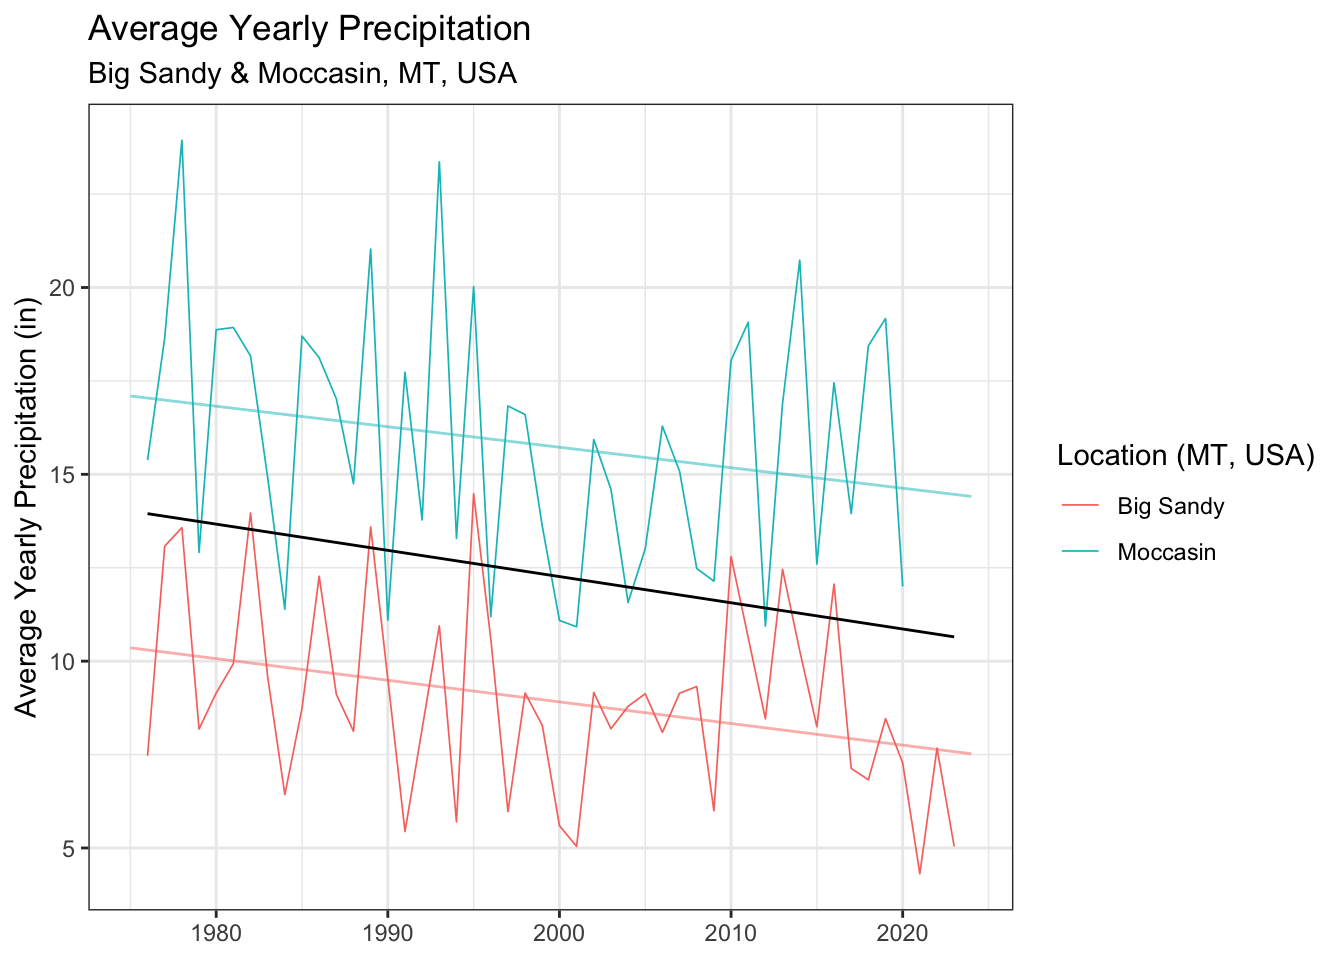
\includegraphics{paper1_files/figure-latex/both_prcp_plot_show-1.pdf}

In addition, we observed a significant positive linear relationship
(\emph{r = 0.178, P \textless{} 0.05, estimate = 0.024}) between year
and average yearly temperature for Moccasin, MT. This means that each
year, the average daily temperature has increased by 0.02°F.

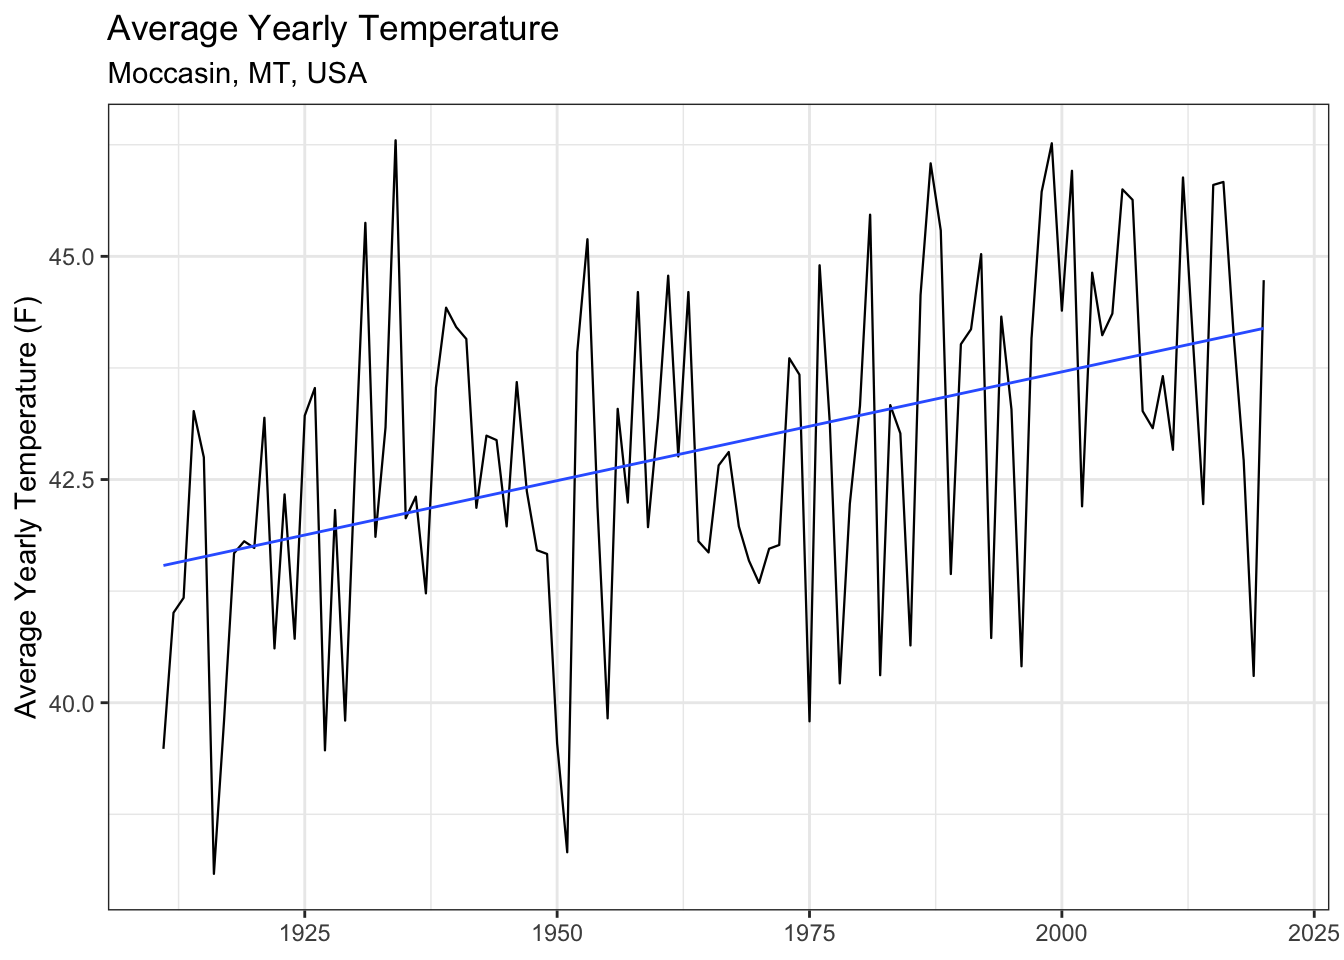
\includegraphics{paper1_files/figure-latex/moc_temp_plot_show-1.pdf}

\subsubsection{NDVI Analysis of Field
Sites}\label{ndvi-analysis-of-field-sites}

We observed a notable difference in NDVI when comparing adjacent
\emph{B. inermis} and spring wheat. We saw a significant difference in
the July NDVI (\emph{0.846, P \textless{} 0.05}). The \emph{B. inermis}
NDVI remained relatively linear in it's downslope (BROME SLOPE POST
JULY) compared to the wheat field (WHEAT FIELD POST JULY).

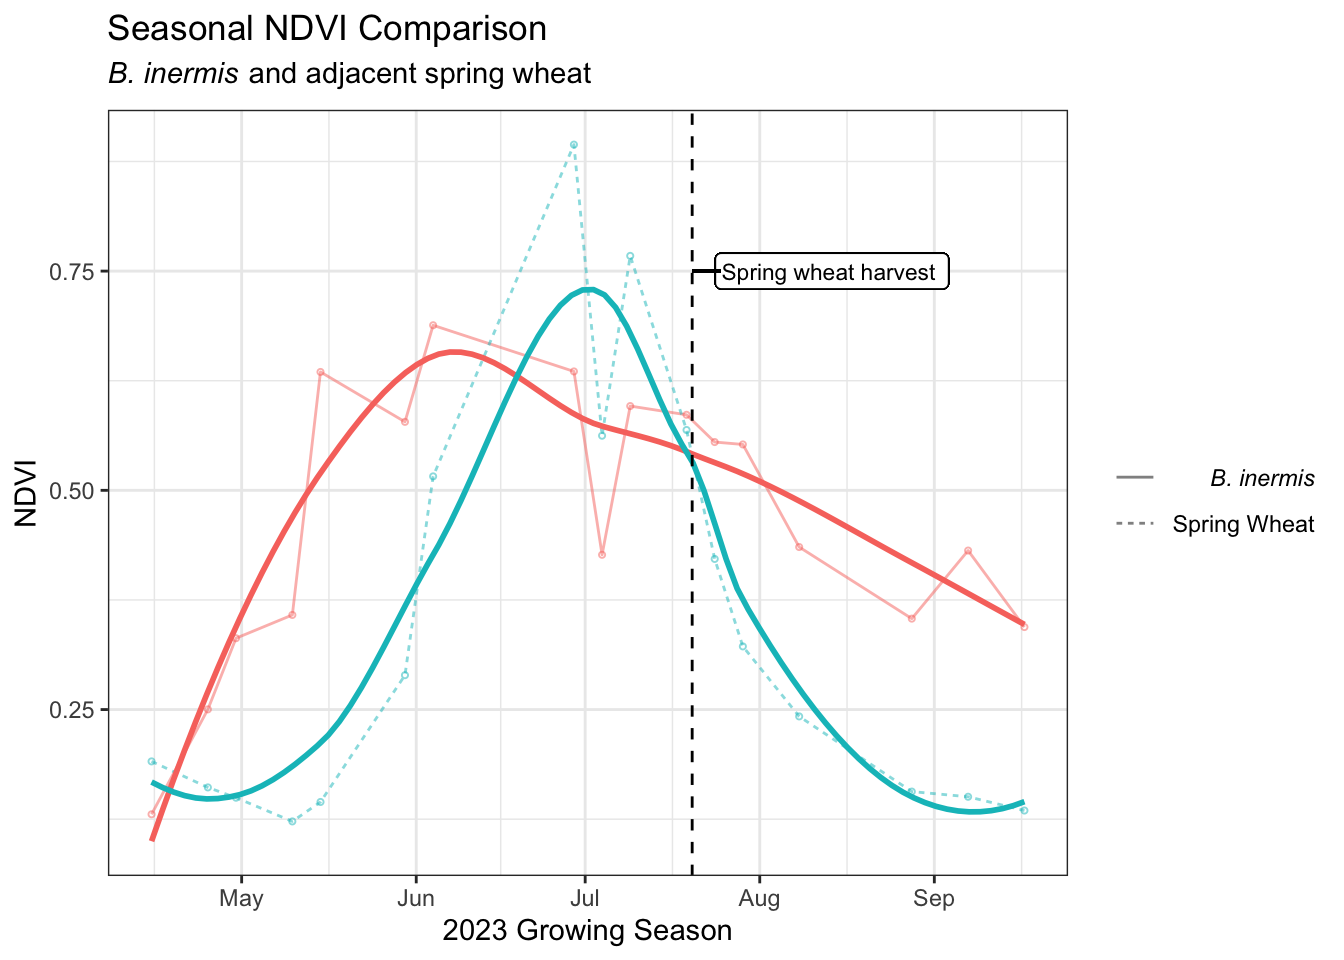
\includegraphics{paper1_files/figure-latex/bs_ndvi_plot-1.pdf}

Need to add map showing where NDVI measurments came from

\subsubsection{\texorpdfstring{Controlled \emph{C cinctus} Infestation
of \emph{B.
inermis}}{Controlled C cinctus Infestation of B. inermis}}\label{controlled-c-cinctus-infestation-of-b.-inermis}

\emph{C. cinctus} showed a high ability to infest \emph{B. inermis} in
the controlled test conditions. Averaged across both years, we observed
66.5\% of stems infested for high treatments and 47.3\% of stems for low
treatments. We found strong evidence suggesting that there was a
significant difference between infestation at high and low treatment
levels when holding year constant (\emph{r = 0.83, P \textless{} 0.05}).

Cutting was observed at 5.7\% for the high treatments and 3.9\% for the
low, showing strong evidence for a difference in cutting between high
and low treatment groups (\emph{r = 0.592, P \textless{} 0.05}).

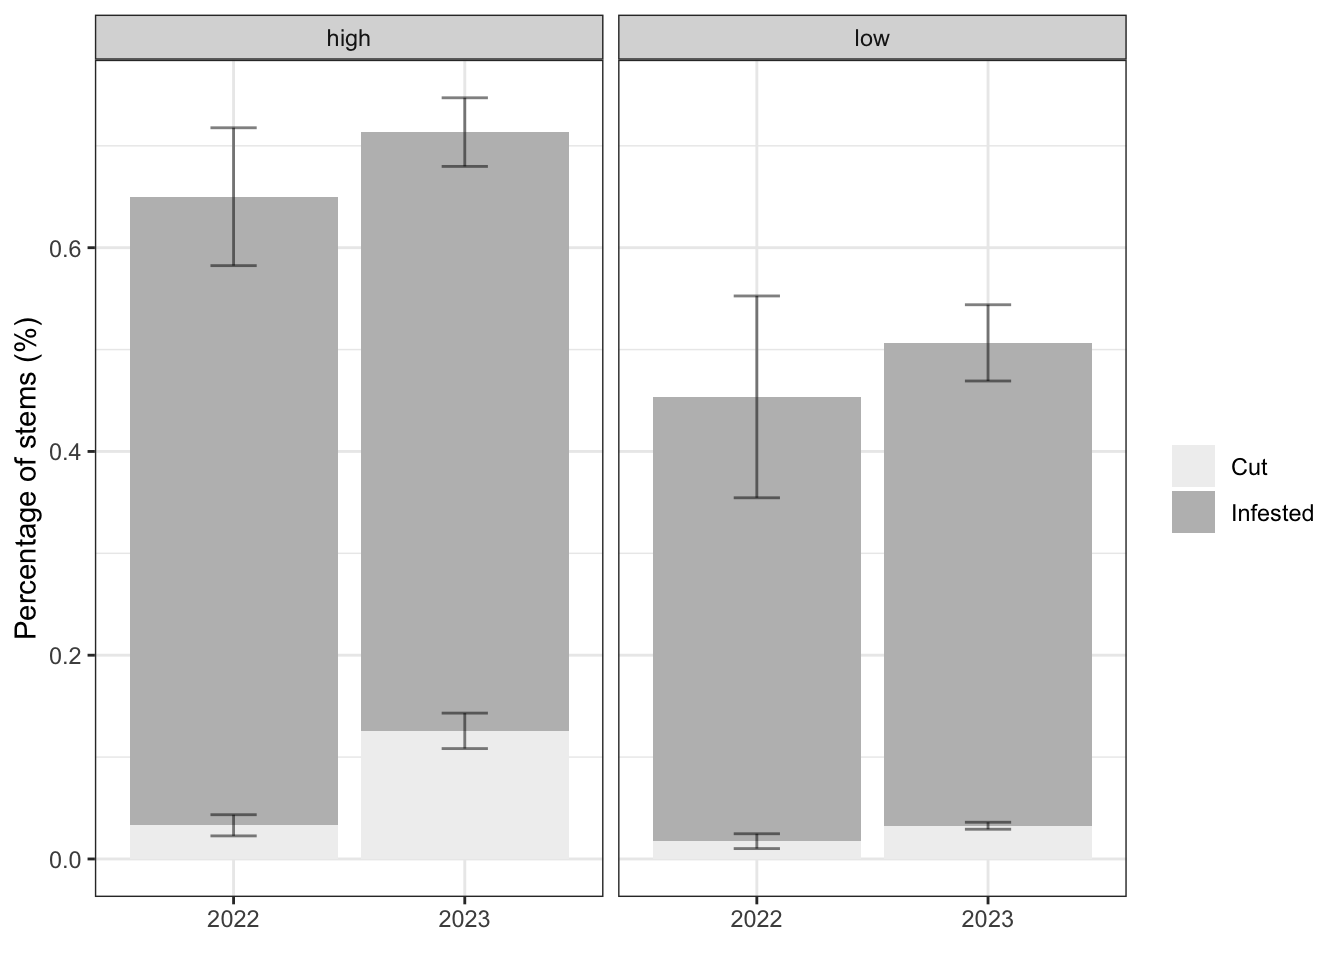
\includegraphics{paper1_files/figure-latex/inf_cut_plot-1.pdf}

\subsubsection{Montana Field Sites}\label{montana-field-sites}

We quantified \emph{C. cinctus} and \emph{Bracon} spp. parasitoid
presence in 6,148 wheat and grass stems across 10 research sites in 2022
and 2023. Infestation by \emph{C. cinctus} within \emph{B. inermis}
varied between collection sites, with the greatest infestation taking
place within our three Big Sandy, MT sampling sites (2023: 65.4\%, 2022:
63.1\%), while the lowest infestation observed was in Moccasin, MT
(2023: 40.8\%, 2022: 60.7\%). Across all sites in Big Sandy and
Moccasin, we observed an average infestation of 57.5\% within \emph{B.
inermis} and 47.6\% within the adjacent wheat.

Parasitoid presence was observed at the highest levels in

\emph{B. inermis} displayed very low levels of \emph{C. cinctus} cutting
when compared to adjacent wheat fields. In Moccasin,

\begin{verbatim}
## [1] 6148
\end{verbatim}

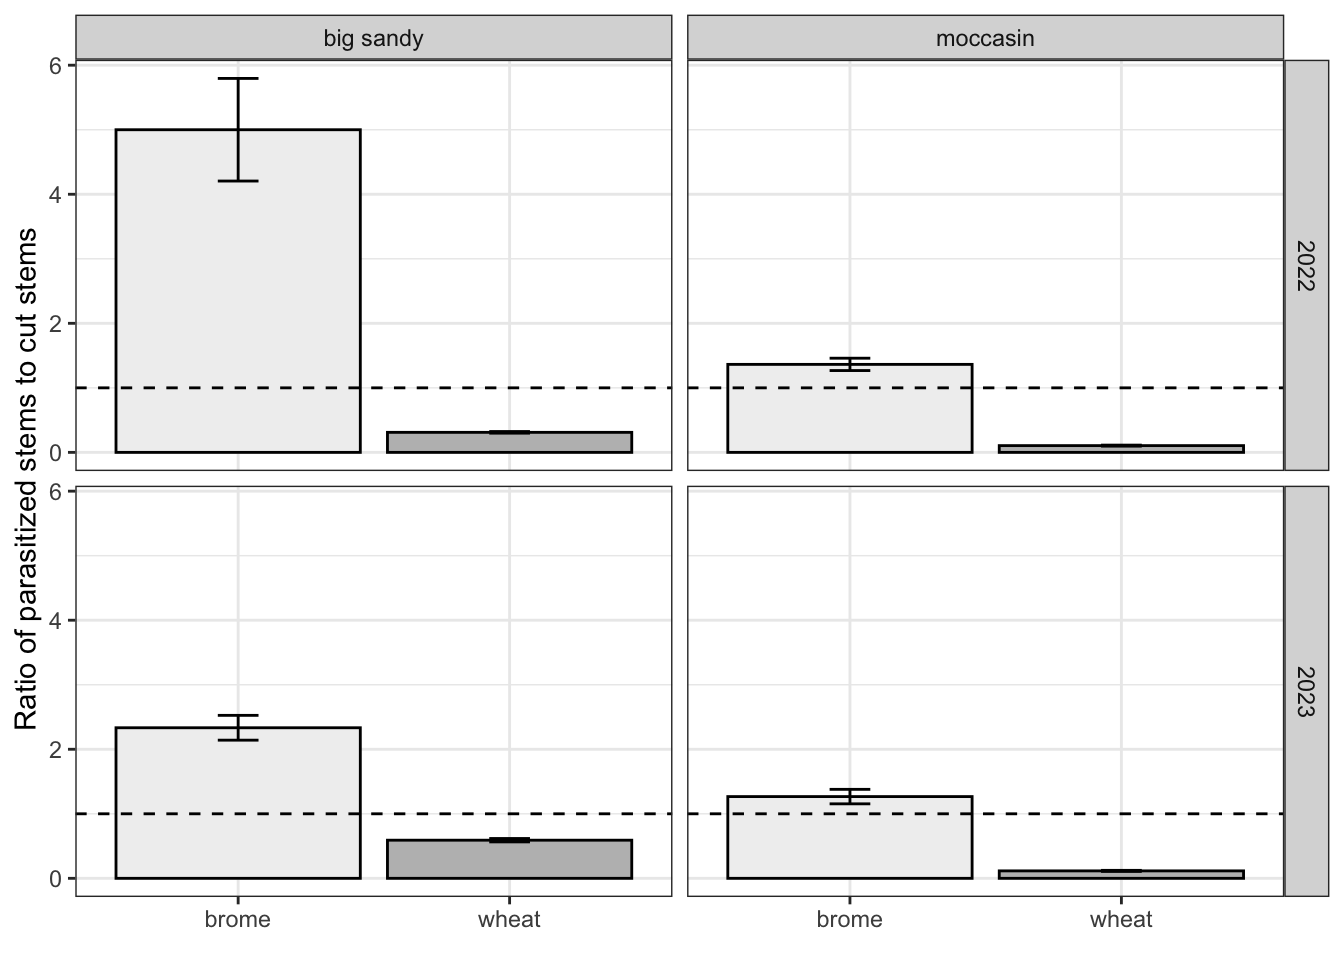
\includegraphics{paper1_files/figure-latex/plot ratios with error bars-1.pdf}

Big Sandy

Turn: 3m x 17m = 51\(m^2\)

North Road North: 5m x 20m = 100\(m^2\)

North Road South: 5m x 20m = 200\(m^2\)

Each sample: 1\(m^2\)

Wheat field sampled area 4 rows, 10 meters between each row samples
taken at 5 and 20 distance from the edge This means the area of the
sampled area is 20x4m = 80\(m^2\) Each sample we'll count as 1m x 0.5m =
0.5\(m^2\) This means 160 possible samples from the sampling area.

Big Sandy NN Brome: 100\(m^2\) - number of Wheat: 80\(m^2\)

Just need the density per unit area. don't need the total number of
p-toids in the entire sampling area.

Just need to standardize it to area so that the sampling size of wheat
is the same as brome. These were different in the field. Brome: 1\(m^2\)
wheat: 0.5\(m^2\)

Also need: - weather data to see if there is a drought causing
crashes/spikes - NDVI data to show greening of brome compared to wheat
late in the season

\subsection*{Citations}\label{citations}
\addcontentsline{toc}{subsection}{Citations}

\phantomsection\label{refs}
\begin{CSLReferences}{1}{0}
\bibitem[\citeproctext]{ref-lme4}
Douglas Bates, MM, Ben Bolker, and Steve Walker. 2015. {``Fitting Linear
Mixed-Effects Models Using Lme4.''} \emph{Journal of Statistical
Software} 67 (1): 1--48.

\bibitem[\citeproctext]{ref-Pettorelli2005}
Pettorelli, Nathalie, Jon Olav Vik, Atle Mysterud, Jean Michel Gaillard,
Compton J. Tucker, and Nils Chr Stenseth. 2005. {``Using the
Satellite-Derived NDVI to Assess Ecological Responses to Environmental
Change.''} \emph{Trends in Ecology and Evolution}.
\url{https://doi.org/10.1016/j.tree.2005.05.011}.

\bibitem[\citeproctext]{ref-ggplot}
Wickham, Hadley. 2016. \emph{Ggplot2: Elegant Graphics for Data
Analysis}. Springer-Verlag New York.
\url{https://ggplot2.tidyverse.org}.

\end{CSLReferences}

\end{document}
